% Emacs, this is -*-latex-*-

\ex{Visualising and analysing Gibbs distributions via undirected graphs}
\label{ex:visualising-gibbs-distributions}
We here consider the Gibbs distribution
$$p(x_1, \ldots, x_5) \propto \phi_{12}(x_1,x_2)\phi_{13}(x_1,x_3)\phi_{14}(x_1,x_4)\phi_{23}(x_2,x_3)\phi_{25}(x_2,x_5)\phi_{45}(x_4,x_5)$$

\begin{exenumerate}
\item Visualise it as an undirected graph.

  \begin{solution}

   We draw a node for each random variable $x_i$. There is an edge between two nodes if the corresponding variables co-occur in a factor.
\begin{center}
\scalebox{0.9}{
\begin{tikzpicture}[ugraph]

\node[cont] (x1) at (0,0) {$x_1$};
\node[cont] (x2) at (2,1) {$x_2$};
\node[cont] (x3) at (1,2) {$x_3$};
\node[cont] (x4) at (4,0) {$x_4$};
\node[cont] (x5) at (3,2) {$x_5$};

\draw(x1) -- (x2);
\draw(x1) -- (x3);
\draw(x1) -- (x4);
\draw(x2) -- (x3);
\draw(x2) -- (x5);
\draw(x4) -- (x5);

\end{tikzpicture}}
\end{center}

  \end{solution}

\item What are the neighbours of $x_3$ in the graph?

  \begin{solution}
    The neighbours are all the nodes for which there is a single connecting edge. Thus:
    $\ne(x_3) = \{x_1, x_2\}$. (Note that sometimes, we may denote $\ne(x_3)$ by $\ne_3$.)
  \end{solution}

\item Do we have $x_3 \independent x_4 \mid x_1, x_2$?

  \begin{solution}
    Yes. The conditioning set $\{x_1,x_2\}$ equals $\ne_3$, which is also the Markov blanket of  $x_3$. This means that $x_3$ is conditionally independent of all the other variables given $\{x_1,x_2\}$, i.e.\ $x_3 \independent x_4,x_5 \mid x_1, x_2$, which implies that $x_3 \independent x_4 \mid x_1, x_2$. (One can also use graph separation to answer the question.)
  \end{solution}

\item What is the Markov blanket of $x_4$?

  \begin{solution}

    The Markov blanket of a node in a undirected graphical model equals the set of its neighbours: $\MB(x_4) = \ne(x_4) = \ne_4 = \{x_1,x_5\}$.  This implies, for example, that
    $x_4 \independent x_2,x_3 \mid x_1,x_5$.
  \end{solution}

\item On which minimal set of variables $A$ do we need to condition to have $x_1 \independent x_5 \mid A$?

  \begin{solution}
We first identify all trails from $x_1$ to $x_5$. There are three such trails: $(x_1,x_2,x_5)$, $(x_1, x_3, x_2, x_5)$, and $(x_1,x_4, x_5)$. Conditioning on $x_2$ blocks the first two trails, conditioning on $x_4$ blocks the last. We thus have: $x_1 \independent x_5 \mid x_2,x_4$, so that $A=\{x_2,x_4\}$.

\end{solution}

\end{exenumerate}

% --------------------------------------------------

\ex{Factorisation and independencies for undirected graphical models}
\label{ex:factorisation-independencies-undirected-graphical-model}
Consider the undirected graphical model defined by the graph in Figure \ref{fig:undirected-graphical-model}.
  \begin{figure}[h]
  \begin{center}
   \scalebox{0.9}{ % x,y
     \begin{tikzpicture}[ugraph]
       \node[cont] (x1) at (0,0) {$x_1$};
       \node[cont] (x2) at (0,-2) {$x_2$};
       \node[cont] (x3) at (2,0) {$x_3$};
       \node[cont] (x4) at (2,-2) {$x_4$};
       \node[cont] (x5) at (3,-1) {$x_5$};
       \node[cont] (x6) at (5,-2) {$x_6$};
       \draw(x1) -- (x3);
       \draw(x1) -- (x2);
       \draw(x2) -- (x4);
       \draw(x1) -- (x4);
       \draw(x3) -- (x4);
       \draw(x3) -- (x5);
       \draw(x4) -- (x5);
       \draw(x5) -- (x6);
       \draw(x4) -- (x6);
   \end{tikzpicture}}
  \end{center}
  \caption{\label{fig:undirected-graphical-model} Graph for \exref{ex:factorisation-independencies-undirected-graphical-model}}
\end{figure}

\begin{exenumerate}


\item What is the set of Gibbs distributions that is induced by the graph?

  \begin{solution}
  The graph in Figure \ref{fig:undirected-graphical-model} has four maximal cliques:
  $$(x_1,x_2,x_4) \quad (x_1,x_3,x_4) \quad (x_3,x_4,x_5) \quad (x_4, x_5, x_6)$$
  The Gibbs distributions are thus
  $$p(x_1,\ldots,x_6) \propto \phi_1(x_1,x_2,x_4) \phi_2(x_1,x_3,x_4) \phi_3(x_3,x_4,x_5) \phi_4(x_4, x_5, x_6)$$
\end{solution}

\item Let $p$ be a pdf that factorises according to the graph. Does $p(x_3 | x_2, x_4) = p(x_3 | x_4)$ hold?

  \begin{solution}
    $p(x_3 | x_2, x_4) = p(x_3 | x_4)$ means that $x_3 \independent
    x_2 \mid x_4$. We can use the graph to check whether this
    generally holds for pdfs that factorise according to the
    graph. There are multiple trails from $x_3$ to $x_2$, including
    the trail $(x_3,x_1,x_2)$, which is not blocked by $x_4$. From the
    graph, we thus cannot conclude that $x_3 \independent x_2 \mid x_4$,
    and $p(x_3 | x_2, x_4) = p(x_3 | x_4)$ will generally not hold
    (the relation may hold for some carefully defined factors $\phi_i$).

  \end{solution}

\item Explain why $x_2 \independent x_5 \mid x_1,x_3,x_4,x_6$ holds for all distributions that factorise over the graph.

  \begin{solution}
    Distributions that factorise over the graph satisfy the pairwise Markov property. Since $x_2$ and $x_5$ are not neighbours, and $x_1,x_3,x_4,x_6$
    are the remaining nodes in the graph, the independence relation follows from the pairwise Markov property.
  \end{solution}

\item Assume you would like to approximate $\E (x_1 x_2 x_5 \mid
  x_3,x_4)$, i.e.\ the expected value of the product of $x_1$, $x_2$,
  and $x_5$ given $x_3$ and $x_4$, with a sample average. Do you
  need to have joint observations for all five variables $x_1, \ldots, x_5$?

  \begin{solution}

    In the graph, all trails from $\{x_1,x_2\}$ to $x_5$ are blocked by $\{x_3,x_4\}$, so that $x_1, x_2 \independent x_5 \mid x_3, x_4$. We thus have
    $$\E (x_1 x_2 x_5 \mid x_3,x_4) =  \E (x_1 x_2 \mid x_3,x_4)  \E (x_5 \mid x_3,x_4).$$
    Hence, we only need joint observations of $(x_1, x_2, x_3, x_4)$ and $(x_3, x_4,x_5)$. Variables $(x_1,x_2)$ and $x_5$ do not need to be jointly measured.

  \end{solution}

\end{exenumerate}


% -----------------------------------------
\ex{Factorisation and independencies for undirected graphical models}
\label{ex:factorisation-independencies-diamond}

Consider the undirected graphical model defined by the following graph, sometimes called a diamond configuration.

\begin{center}
  \scalebox{1}{ % w,x,y,z
    \begin{tikzpicture}[ugraph]
      \node[cont] (w) at (0,1) {$w$};
      \node[cont] (x) at (1,2) {$x$};
      \node[cont] (y) at (2,1) {$y$};
      \node[cont] (z) at (1,0) {$z$};
      \draw(w) -- (x);
      \draw(w) -- (z);
      \draw(x) -- (y);
      \draw(y) -- (z);
    \end{tikzpicture}
  }
\end{center}

\begin{exenumerate}

\item How do the pdfs/pmfs of the undirected graphical model factorise?

  \begin{solution}
    The maximal cliques are $(x, w)$, $(w, z)$, $(z, y)$ and $(x,
    y)$. The undirected graphical model thus consists of pdfs/pmfs
    that factorise as follows
    \begin{equation}
      p(x, w, z, y) \propto \phi_1(x,w) \phi_2(w,z) \phi_3(z,y) \phi_4(x,y)
    \end{equation}

  \end{solution}

\item List all independencies that hold for the undirected graphical model.

  \begin{solution}
    We can generate the independencies by conditioning on
    progressively larger sets. Since there is a trail between any two
    nodes, there are no unconditional independencies. If we condition
    on a single variable, there is still a trail that connects the
    remaining ones. Let us thus consider the case where we condition
    on two nodes. By graph separation, we have
    \begin{equation}
      w \independent y \mid x,z \quad \quad x \independent z \mid w,y
    \end{equation}
    These are all the independencies that hold for the model, since
    conditioning on three nodes does not lead to any independencies in
    a model with four variables.
  \end{solution}


\end{exenumerate}

% --------------------------------------------------

\ex{Factorisation from the Markov blankets I}
\label{ex:factorisation-from-the-Markov-blankets-I}

Assume you know the following Markov blankets for all variables $x_1,
\ldots, x_4, y_1, \ldots y_4$ of a pdf or pmf $p(x_1, \ldots, x_4,
y_1, \ldots,y_4)$.
\begin{align}
  \MB(x_1) &= \{x_2, y_1\} & \MB(x_2)&=\{x_1, x_3, y_2\} & \MB(x_3)&=\{x_2, x_4, y_3\} & \MB(x_4)&=\{x_3, y_4\}\\
  \MB(y_1) &= \{x_1\}      & \MB(y_2)&= \{x_2\}         &  \MB(y_3)&= \{x_3\}         &  \MB(y_4) &= \{x_4\}
\end{align}
Assuming that $p$ is positive for all possible
values of its variables, how does $p$ factorise?

\begin{solution}
In undirected graphical models, the Markov blanket for a variable is
the same as the set of its neighbours. Hence, when we are given all
Markov blankets we know what local Markov property $p$ must
satisfy. For positive distributions we have an equivalence between $p$
satisfying the local Markov property and $p$ factorising over the
graph. Hence, to specify the factorisation of $p$ it suffices to
construct the undirected graph $H$ based on the Markov blankets and
then read out the factorisation.

We need to build a graph where the neighbours of each variable equals
the indicated Markov blanket. This can be easily done by starting with
an empty graph and connecting each variable to the variables in its
Markov blanket.

We see that each $y_i$ is only connected to $x_i$. Including those
Markov blankets we get the following graph:

\begin{center}
  \scalebox{1}{
    \begin{tikzpicture}[ugraph]
      \node[cont] (y1) at (0,0) {$y_1$};
      \node[cont] (y2) at (2,0) {$y_2$};
      \node[cont] (y3) at (4,0) {$y_3$};
      \node[cont] (y4) at (6,0) {$y_4$};
      \node[cont] (x1) at (0,2) {$x_1$};
      \node[cont] (x2) at (2,2) {$x_2$};
      \node[cont] (x3) at (4,2) {$x_3$};
      \node[cont] (x4) at (6,2) {$x_4$};
      \draw(x1)--(y1);\draw(x2)--(y2);\draw(x3)--(y3);\draw(x4)--(y4);
  \end{tikzpicture}}
\end{center}

Connecting the $x_i$ to their neighbours according to the Markov blanket thus gives:

\begin{center}
  \scalebox{1}{
    \begin{tikzpicture}[ugraph]
      \node[cont] (y1) at (0,0) {$y_1$};
      \node[cont] (y2) at (2,0) {$y_2$};
      \node[cont] (y3) at (4,0) {$y_3$};
      \node[cont] (y4) at (6,0) {$y_4$};
      \node[cont] (x1) at (0,2) {$x_1$};
      \node[cont] (x2) at (2,2) {$x_2$};
      \node[cont] (x3) at (4,2) {$x_3$};
      \node[cont] (x4) at (6,2) {$x_4$};
      \draw(x1)--(y1);\draw(x2)--(y2);\draw(x3)--(y3);\draw(x4)--(y4);
      \draw(x1)--(x2);\draw(x2)--(x3);\draw(x3)--(x4);
  \end{tikzpicture}}
\end{center}

The graph has maximal cliques of size two, namely the $x_i-y_i$ for
$i=1,\ldots, 4$, and the $x_i-x_{i+1}$ for $i=1, \ldots, 3$.  Given
the equivalence between the local Markov property and factorisation
for positive distributions, we know that $p$ must factorise as
\begin{align}
  p(x_1, \ldots, x_4, y_1, \ldots, y_4) = \frac{1}{Z} \prod_{i=1}^3 m_i(x_i,x_{i+1}) \prod_{i=1}^4 g_i(x_i,y_i),
\end{align}
where $m_i(x_i, x_{i+1})>0$, $g(x_i,y_i)>0$ are positive factors (potential functions).

The graphical model corresponds to an undirected version of a hidden
Markov model where the $x_i$ are the unobserved (latent, hidden)
variables and the $y_i$ are the observed ones. Note that the $x_i$
form a Markov chain.

\end{solution}

\ex{Factorisation from the Markov blankets II}
\label{ex:factorisation-from-the-Markov-blankets-II}

We consider the same setup as in Exercise \ref{ex:factorisation-from-the-Markov-blankets-I} but we now assume that we do not know all Markov blankets but only
\begin{align}
  \MB(x_1) &= \{x_2, y_1\} & \MB(x_2)&=\{x_1, x_3, y_2\} & \MB(x_3)&=\{x_2, x_4, y_3\} & \MB(x_4)&=\{x_3, y_4\}
\end{align}
Without inserting more independencies than those specified by the
Markov blankets, draw the graph over which $p$ factorises and state
the factorisation. (Again assume that $p$ is positive for all possible
values of its variables).

\begin{solution}
We take the same approach as in Exercise
\ref{ex:factorisation-from-the-Markov-blankets-I}. In particular, the
Markov blankets of a variable are its neighbours in the graph. But
since we are not given all Markov blankets and are not allowed to
insert additional independencies, we must assume that each $y_i$ is
connected to all the other $y$'s. For example, if we didn't connect
$y_1$ and $y_4$ we would assert the additional independency $y_1
\independent y_4 \mid x_1,x_2,x_3,x_4,y_2,y_3$.

We thus have a graph as follows:

\begin{center}
  \scalebox{1}{
    \begin{tikzpicture}[ugraph]
      \node[cont] (y1) at (0,0) {$y_1$};
      \node[cont] (y2) at (2,0) {$y_2$};
      \node[cont] (y3) at (4,0) {$y_3$};
      \node[cont] (y4) at (6,0) {$y_4$};
      \node[cont] (x1) at (0,2) {$x_1$};
      \node[cont] (x2) at (2,2) {$x_2$};
      \node[cont] (x3) at (4,2) {$x_3$};
      \node[cont] (x4) at (6,2) {$x_4$};
      \draw(x1)--(y1);\draw(x2)--(y2);\draw(x3)--(y3);\draw(x4)--(y4);
      \draw(x1)--(x2);\draw(x2)--(x3);\draw(x3)--(x4);
      \draw(y1)--(y2);\draw(y1) to [bend right= 45] (y3);\draw(y1)  to [bend right= 45] (y4);
      \draw(y2)--(y3);\draw(y2) to [bend right=45]  (y4);\draw(y3)--(y4);
  \end{tikzpicture}}
\end{center}

The factorisation thus is
\begin{align}
  p(x_1, \ldots, x_4, y_1, \ldots, y_4) = \frac{1}{Z} g(y_1, \ldots, y_4) \prod_{i=1}^3 m_i(x_i,x_{i+1})\prod_{i=1}^4 g_i(x_i,y_i),
\end{align}
where the $m_i(x_i, x_{i+1})$, $g_i(x_i, y_i)$ and $g(y_1, \ldots, y_4)$ are positive
factors. Compared to the factorisation in Exercise
\ref{ex:factorisation-from-the-Markov-blankets-I}, we still have the
Markov structure for the $x_i$, but only a single factor for $(y_1,
y_2, y_3, y_4)$ to avoid inserting independencies beyond those
specified by the given Markov blankets.


\end{solution}


% ------------------------------------------------

\ex{Undirected graphical model with pairwise potentials}
We here consider Gibbs distributions where the factors only depend on two variables at
a time. The probability density or mass functions over $d$ random
variables $x_1, \ldots, x_d$ then take the form
$$p(x_1, \ldots, x_d) \propto \prod_{i \le j} \phi_{ij}(x_i,x_j)$$
Such models are sometimes called pairwise Markov networks.

\begin{exenumerate}

\item Let $p(x_1, \ldots, x_d) \propto \exp\left( -\frac{1}{2} \x^\top
  \A \x - \b^\top \x \right)$ where $\A$ is symmetric and $\x = (x_1,
  \ldots, x_d)^\top$. What are the corresponding factors $\phi_{ij}$
  for $i\le j$?
  \begin{solution}
    Denote the $(i,j)$-th element of $\A$ by $a_{ij}$. We have
    \begin{align}
      \x^\top \A \x & = \sum_{ij} a_{ij} x_i x_j \\
      &= \sum_{i<j} 2 a_{ij} x_i x_j + \sum_i a_{ii} x_i^2
    \end{align}
    where the second line follows from $\A^\top =\A$. Hence,
    \begin{align}
      -\frac{1}{2} \x^\top \A \x - \b^\top \x & = -\frac{1}{2} \sum_{i<j} 2a_{ij} x_i x_j - \frac{1}{2} \sum_i a_{ii} x_i^2 - \sum_i b_i x_i
    \end{align}
    so that
\begin{equation}
      \phi_{ij}(x_i,x_j) = \begin{cases}
        \exp\left(- a_{ij} x_i x_j\right) & \text{if } i < j\\
        \exp\left( - \frac{1}{2} a_{ii} x_i^2 - b_i x_i\right) & \text{if } i=j
      \end{cases}
      \label{eq:pairwisepot}
\end{equation}
For $\x \in \mathbb{R}^d$, the distribution is a Gaussian with $\A$
equal to the inverse covariance matrix. For binary $\x$, the model is
known as Ising model or Boltzmann machine. For $x_i \in \{-1,1\}$,
$x_i^2=1$ for all $i$, so that the $a_{ii}$ are constants
that can be absorbed into the normalisation constant. This means that
for $x_i \in \{-1,1\}$, we can work with matrices $\A$ that have zeros
on the diagonal.

  \end{solution}

\item For $p(x_1, \ldots, x_d) \propto \exp\left( -\frac{1}{2} \x^\top
  \A \x - \b^\top \x \right)$, show that $x_i \independent x_j \mid
  \{x_1, \ldots, x_d\} \setminus \{x_i,x_j\}$ if the $(i,j)$-th
  element of $\A$ is zero.

  \begin{solution}

    The previous question showed that we can write $p(x_1, \ldots,
    x_d) \propto \prod_{i \leq j} \phi_{ij}(x_i,x_j)$ with potentials as in
    Equation \eqref{eq:pairwisepot}.  Consider two variables $x_i$ and
    $x_j$ for fixed $(i,j)$. They only appear in the factorisation via
    the potential $\phi_{ij}$. If $a_{ij} = 0$, the factor $\phi_{ij}$
    becomes a constant, and no other factor contains $x_i$ and $x_j$,
    which means that there is no edge between $x_i$ and $x_j$ if
    $a_{ij}=0$. By the pairwise Markov property it then follows that
    $x_i \independent x_j \mid \{x_1, \ldots, x_d\} \setminus \{x_i,x_j\}$.

  \end{solution}

\end{exenumerate}


% ---------------------------------------------------------------

\ex{Restricted Boltzmann machine {\small \citep[based on][Exercise 4.4]{Barber2012}}}%
The restricted Boltzmann machine is an undirected
graphical model for binary variables $\v =(v_1, \ldots, v_n)^\top$ and
$\h=(h_1, \ldots, h_m)^\top$ with a probability mass function equal to
\begin{equation}
  p(\v,\h) \propto \exp\left( \v^\top \W \h + \a^\top\v + \b^\top\h \right),
\end{equation}
where $\W$ is a $n \times m$ matrix. Both the $v_i$ and $h_i$ take values in $\{0,1\}$. The
$v_i$ are called the ``visibles'' variables since they are assumed to
be observed while the $h_i$ are the hidden variables since it is
assumed that we cannot measure them.

\begin{exenumerate}
\item Use graph separation to show that the joint conditional $p(\h | \v)$ factorises as
  $$p(\h | \v) = \prod_{i=1}^m p(h_i | \v).$$

  \begin{solution}
    Figure \ref{fig:restricted-boltzmann-machine} on the left shows
    the undirected graph for $p(\v,\h)$ with $n=3, m=2$. We note that
    the graph is bi-partite: there are only direct connections
    between the $h_i$ and the $v_i$. Conditioning on $\v$ thus blocks
    all trails between the $h_i$ (graph on the right). This means that
    the $h_i$ are independent from each other given $\v$ so that
    $$p(\h | \v) = \prod_{i=1}^m p(h_i | \v).$$

    \begin{figure}[ht]
      \centering
      \scalebox{1}{
        \begin{tikzpicture}[ugraph]

          \node[cont] (h1) at (-1,0) {$h_1$};
          \node[cont] (h2) at (1,0) {$h_2$};
          \node[cont] (v1) at (-2,-2) {$v_1$};
          \node[cont] (v2) at (0,-2) {$v_2$};
          \node[cont] (v3) at (2,-2) {$v_3$};

          \draw(h1) -- (v1);
          \draw(h1) -- (v2);
          \draw(h1) -- (v3);
          \draw(h2) -- (v1);
          \draw(h2) -- (v2);
          \draw(h2) -- (v3);

          % -----------------

          \node[cont] (h1) at (7,0) {$h_1$};
          \node[cont] (h2) at (9,0) {$h_2$};
          \node[contobs] (v1) at (6,-2) {$v_1$};
          \node[contobs] (v2) at (8,-2) {$v_2$};
          \node[contobs] (v3) at (10,-2) {$v_3$};

          \draw(h1) -- (v1);
          \draw(h1) -- (v2);
          \draw(h1) -- (v3);
          \draw(h2) -- (v1);
          \draw(h2) -- (v2);
          \draw(h2) -- (v3);

      \end{tikzpicture}}
      \caption{\label{fig:restricted-boltzmann-machine} Left: Graph for $p(\v,\h)$. Right: Graph for $p(\h | \v)$}
    \end{figure}
  \end{solution}

\item Show that
  \begin{equation}
    p(h_i = 1 | \v) = \frac{1}{1+\exp\left(-b_i-\sum_j W_{ji} v_j\right)}
    \label{eq:hcondv}
  \end{equation}
where $W_{ji}$ is the $(ji)$-th element of $\W$, so that $\sum_j W_{ji} v_j$ is the inner product (scalar product) between the $i$-th column of $\W$ and $\v$.
    \begin{solution}

     For the conditional pmf $p(h_i | \v)$ any quantity that does not
     depend on $h_i$ can be considered to be part of the normalisation constant. A general strategy is to first work out $p(h_i | \v)$ up to the normalisation constant and then to normalise it afterwards.

     We begin with $p(\h | \v)$:
      \begin{align}
        p(\h | \v) &= \frac{p(\h,\v)}{p(\v)} \\
        & \propto p(\h,\v) \\
        & \propto \exp\left( \v^\top \W \h + \a^\top\v + \b^\top\h \right)\\
        & \propto \exp\left( \v^\top \W \h + \b^\top\h \right)\\
        & \propto \exp\left( \sum_i \sum_j v_j W_{ji} h_i + \sum_i b_i h_i \right)
     \end{align}
     As we are interested in $p(h_i | \v)$ for a fixed $i$, we can drop all the terms not depending on that $h_i$, so that
      \begin{align}
        p(h_i | \v) & \propto \exp\left( \sum_j v_j W_{ji} h_i + b_i h_i \right)
      \end{align}
      Since $h_i$ only takes two values, 0 and 1, normalisation is here straightforward. Call the unnormalised pmf $\tilde{p}(h_i | \v)$,
      \begin{equation}
        \tilde{p}(h_i | \v) = \exp\left( \sum_j v_j W_{ji} h_i + b_i h_i \right).
      \end{equation}
      We then have
      \begin{align}
        p(h_i | \v) &= \frac{\tilde{p}(h_i | \v)} { \tilde{p}(h_i=0 | \v) + \tilde{p}(h_i =1 | \v)}\\
        & = \frac{\tilde{p}(h_i | \v)} { 1+  \exp\left( \sum_j v_j W_{ji} + b_i \right)}\\
        & = \frac{\exp\left( \sum_j v_j W_{ji} h_i + b_i h_i \right)}{ 1+  \exp\left( \sum_j v_j W_{ji} + b_i \right)},
       \end{align}
      so that
      \begin{align}
        p(h_i=1 | \v) & =  \frac{\exp\left( \sum_j v_j W_{ji} + b_i \right)}{ 1+  \exp\left( \sum_j v_j W_{ji} + b_i \right)}\\
         & =  \frac{1}{ 1+  \exp\left(- \sum_j v_j W_{ji} - b_i \right)}.
      \end{align}
      The probability $p(h=0 | \v)$ equals $1 -  p(h_i=1 | \v)$, which is
      \begin{align}
        p(h_i =0 | \v) & =  \frac{1+ \exp\left( \sum_j v_j W_{ji} + b_i \right)}{ 1+  \exp\left( \sum_j v_j W_{ji} + b_i \right)} - \frac{\exp\left( \sum_j v_j W_{ji} + b_i \right)}{ 1+  \exp\left( \sum_j v_j W_{ji} + b_i \right)}\\
        & = \frac{1}{ 1+  \exp\left( \sum_j W_{ji} v_j + b_i \right)}
        \end{align}

      The function $x \mapsto 1/(1+\exp(-x))$ is called the logistic function. It is a sigmoid function and is thus sometimes denoted by $\sigma(x)$.
      For other versions of the sigmoid function, see \url{https://en.wikipedia.org/wiki/Sigmoid_function}.
      \begin{center}
        \vspace{5ex}
        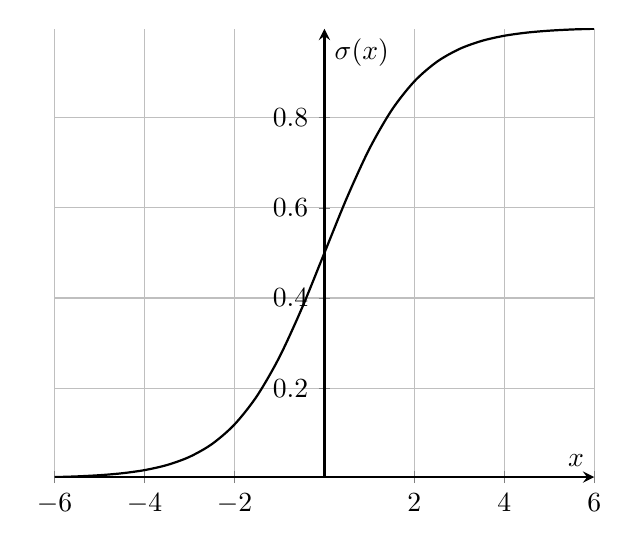
\begin{tikzpicture}
          \begin{axis}[ xlabel={$x$}, ylabel={$\sigma(x)$},
              axis lines=middle, smooth , grid , thick, domain=-6:6]
%          \draw[->] (-5,0) -- (5,0) node[right] {$x$};
%          \draw[->] (0,0) -- (0,1.5) node[above] {$\sigma(x)$};
            \addplot[no marks]{1/(1+exp(-\x))};
            \end{axis}
        \end{tikzpicture}
        \vspace{2ex}
      \end{center}
      With that notation, we have
      \begin{align*}
        p(h_i=1 | \v) &= \sigma\left(\sum_j W_{ji} v_j  + b_i\right).
      \end{align*}

    \end{solution}

  \item Use a symmetry argument to show that
    $$p(\v | \h) = \prod_i p(v_i | \h) \quad \text{ and }  \quad p(v_i = 1 | \h) = \frac{1}{1+\exp\left(-a_i-\sum_j W_{ij} h_j\right)}$$

    \begin{solution}
      Since $\v^\top \W \h$ is a scalar we have  $(\v^\top \W \h)^\top = \h^\top \W^\top \v =  \v^\top \W \h$, so that
      \begin{align}
      p(\v,\h) & \propto \exp\left( \v^\top \W \h + \a^\top\v + \b^\top\h \right) \\
      & \propto \exp\left( \h^\top \W^\top \v + \b^\top\h + \a^\top\v  \right).
      \end{align}
      To derive the result, we note that $\v$ and $a$ now take the place of $\h$ and $\b$ from before, and that we now have $\W^\top$ rather than $\W$. In Equation \eqref{eq:hcondv}, we thus replace $h_i$ with $v_i$, $b_i$ with $a_i$, and $W_{ji}$ with $W_{ij}$ to obtain $p(v_i = 1 | \h)$. In terms of the sigmoid function, we have
       $$ p(v_i=1 | \h) = \sigma\left(\sum_j W_{ij} h_j + a_i\right).$$

      Note that while $p(\v | \h)$ factorises, the marginal $p(\v)$
      does generally not. The marginal $p(\v)$ can here be obtained in
      closed form up to its normalisation constant.
      \begin{align}
        p(\v) & = \sum_{\h \in \{0,1\}^m} p(\v,\h) \\
        & = \frac{1}{Z} \sum_{\h \in \{0,1\}^m} \exp\left( \v^\top \W \h + \a^\top\v + \b^\top\h \right)\\
        & =  \frac{1}{Z}  \sum_{\h \in \{0,1\}^m} \exp\left( \sum_{ij} v_i h_j W_{ij} + \sum_i a_i v_i + \sum_j b_j h_j \right)\\
        & =  \frac{1}{Z}  \sum_{\h \in \{0,1\}^m} \exp\left( \sum_{j=1}^m h_j \left[\sum_i v_i W_{ij} + b_j\right] + \sum_i a_i v_i \right)\\
        & =  \frac{1}{Z}  \sum_{\h \in \{0,1\}^m} \prod_{j=1}^m \exp\left( h_j \left[\sum_i v_i W_{ij} + b_j\right] \right) \exp\left( \sum_i a_i v_i \right)\\
        & =  \frac{1}{Z} \exp\left( \sum_i a_i v_i \right) \sum_{\h \in \{0,1\}^m} \prod_{j=1}^m \exp\left( h_j \left[\sum_i v_i W_{ij} + b_j\right] \right) \\
        & =  \frac{1}{Z} \exp\left( \sum_i a_i v_i \right) \sum_{h_1, \ldots, h_m} \prod_{j=1}^m  \exp\left( h_j \left[\sum_i v_i W_{ij} + b_j\right] \right)
      \end{align}
      Importantly, each term in the product only depends on a single $h_j$, so that by sequentially applying the distributive law, we have
      \begin{align}
        \sum_{h_1, \ldots, h_m} \prod_{j=1}^m  \exp\left( h_j \left[\sum_i v_i W_{ij} + b_j\right] \right)  =& \left[ \sum_{h_1, \ldots, h_{m-1}} \prod_{j=1}^{m-1}  \exp\left( h_j \left[\sum_i v_i W_{ij} + b_j\right] \right)\right] \cdot \nonumber \\
        &\sum_{h_m} \exp\left( h_m \left[\sum_i v_i W_{im} + b_m\right] \right)\\
         =& \ldots \nonumber \\
        =& \prod_{j=1}^m \left[\sum_{h_j} \exp\left( h_j \left[\sum_i v_i W_{ij} + b_j\right] \right)\right]
      \end{align}
      Since $h_j \in \{0,1\}$, we obtain
      \begin{align}
        \sum_{h_j} \exp\left( h_j \left[\sum_i v_i W_{ij} + b_j\right] \right) & = 1+ \exp\left(\sum_i v_i W_{ij} + b_j \right)
      \end{align}
      and thus
       \begin{align}
         p(\v) & = \frac{1}{Z}  \exp\left( \sum_i a_i v_i \right) \prod_{j=1}^m \left[1+ \exp\left(\sum_i v_i W_{ij} + b_j \right)\right].
      \end{align}
       Note that in the derivation of $p(\v)$ we have not used the
       assumption that the visibles $v_i$ are binary. The same
       expression would thus obtained if the visibles were defined in
       another space, e.g.\ the real numbers.

       While $p(\v)$ is written as a product, $p(\v)$ does not
       factorise into terms that depend on subsets of the
       $v_i$. On the contrary, all $v_i$ are present in all
       factors. Since $p(\v)$ does not factorise, computing the
       normalising $Z$ is expensive. For binary visibles
       $v_i \in \{0,1\}$, $Z$ equals
       \begin{equation}
         Z = \sum_{\v \in \{0,1\}^n} \exp\left( \sum_i a_i v_i \right) \prod_{j=1}^m \left[1+ \exp\left(\sum_i v_i W_{ij} + b_j \right)\right]
       \end{equation}
       where we have to sum over all $2^n$ configurations of the
       visibles $\v$. This is computationally expensive, or even
       prohibitive if $n$ is large ($2^{20} = 1048576,\, 2^{30}>
       10^9$). Note that different values of $a_i,b_i,W_{ij}$ yield
       different values of $Z$. (This is a reason why $Z$ is called
       the partition \emph{function} when the $a_i, b_i, W_{ij}$ are free parameters.)

       It is instructive to write $p(\v)$ in the log-domain,
       \begin{align}
         \log p(\v) & = -\log Z + \sum_{i=1}^n a_i v_i + \sum_{j=1}^m \log\left[1+ \exp\left(\sum_i v_i W_{ij} + b_j \right)\right],
       \end{align}
       and to introduce the nonlinearity $f(u)$,
       \begin{align}
         f(u) & = \log\left[ 1+\exp(u) \right],
       \end{align}
       which is called the softplus function and plotted below. The softplus function is a smooth approximation of $\max(0,u)$, see e.g.\ \url{https://en.wikipedia.org/wiki/Rectifier_(neural_networks)}
       \begin{center}
         \vspace{3ex}
         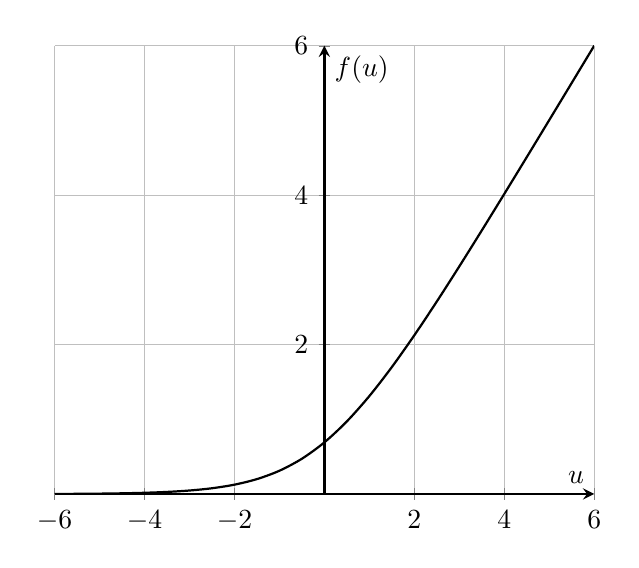
\begin{tikzpicture}
           \begin{axis}[ xlabel={$u$}, ylabel={$f(u)$},
               axis lines=middle, smooth , grid , thick, domain=-6:6]
             %          \draw[->] (-5,0) -- (5,0) node[right] {$x$};
             %          \draw[->] (0,0) -- (0,1.5) node[above] {$\sigma(x)$};
             \addplot[no marks]{ln(1+exp(\x))};
             %\addplot[no marks, red]{max(\x,0)};
           \end{axis}
         \end{tikzpicture}
      \end{center}
       With the softplus function $f(u)$, we can write $\log p(\v)$ as
       \begin{align}
         \log p(\v) & = \log Z + \sum_{i=1}^n a_i v_i + \sum_{j=1}^m f\left(\sum_i v_i W_{ij} + b_j \right).
       \end{align}
       The parameter $b_j$ plays the role of a threshold as shown in
       the figure below. The terms $f\left(\sum_i v_i W_{ij} + b_j
       \right)$ can be interpreted in terms of feature detection. The
       sum $\sum_i v_i W_{ij}$ is the inner product between $\v$ and
       the $j$-th column of $\W$, and the inner product is largest if
       $\v$ equals the $j$-th column. We can thus consider the columns
       of $\W$ to be feature-templates, and the $f\left(\sum_i v_i
       W_{ij} + b_j \right)$ a way to measure how much of each feature
       is present in $\v$.

       Further, $\sum_i v_i W_{ij} +b_j$ is also the input to the
       sigmoid function when computing $p(h_j=1 | \v)$. Thus, the
       conditional probability for $h_j$ to be one, i.e.\ ``active'',
       can be considered to be an indicator of the presence of the
       $j$-th feature ($j$-th column of $\W$) in the input $\v$.

       If $v$ is such that $\sum_i v_i W_{ij} +b_j$ is large for many
       $j$, i.e.\ if many features are detected, then $f\left(\sum_i
       v_i W_{ij} + b_j \right)$ will be non-zero for many $j$, and
       $\log p(\v)$ will be large.


       \begin{center}
         \vspace{3ex}
         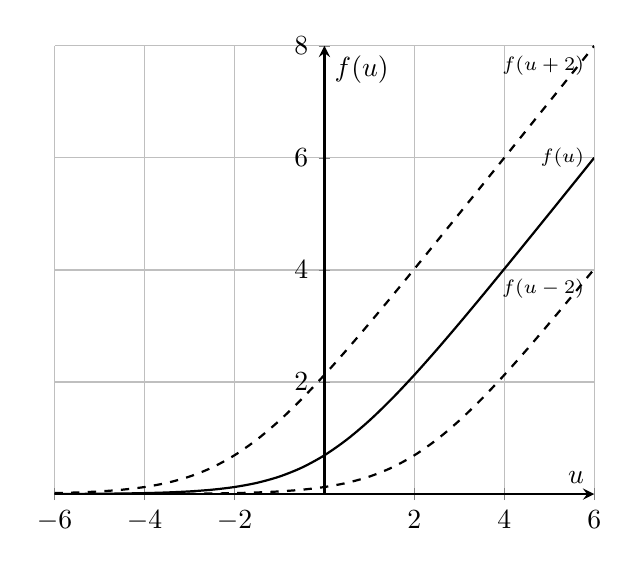
\begin{tikzpicture}
           \begin{axis}[ xlabel={$u$}, ylabel={$f(u)$},
               axis lines=middle, smooth , grid , thick, domain=-6:6]
             %          \draw[->] (-5,0) -- (5,0) node[right] {$x$};
             %          \draw[->] (0,0) -- (0,1.5) node[above] {$\sigma(x)$};
             \addplot[no marks]{ln(1+exp(\x))} node[left]{\scriptsize$f(u)$};
             \addplot[no marks, dashed]{ln(1+exp(\x+2))} node[below left]{\scriptsize $f(u+2)$};
             \addplot[no marks, dashed]{ln(1+exp(\x-2))} node[below left]{\scriptsize $f(u-2)$};
             %\addplot[no marks, red]{max(\x,0)};
           \end{axis}
         \end{tikzpicture}
      \end{center}


    \end{solution}



\end{exenumerate}



\ex{Hidden Markov models and change of measure}

Consider the following undirected graph for a hidden Markov model where the $y_i$ correspond to observed (visible) variables and the $x_i$ to unobserved (hidden/latent) variables.

\begin{center}
  \scalebox{1}{
    \begin{tikzpicture}[ugraph]
      \node[cont] (x1) at (0,2) {$x_1$};
      \node[cont] (x2) at (2,2) {$x_2$};
      \node[cont] (x3) at (4,2) {$x_3$};
      \node       (a) at (6,2) {};
      \node       (b) at (7,2) {$\ldots$};
      \node       (c) at (7,0) {$\ldots$};
      \node       (d) at (8,2) {};
      \node[cont] (x4) at (10,2) {$x_t$};
      \node[cont] (y1) at (0,0) {$y_1$};
      \node[cont] (y2) at (2,0) {$y_2$};
      \node[cont] (y3) at (4,0) {$y_3$};
      \node[cont] (y4) at (10,0) {$y_t$};
      \draw(x1)--(y1);\draw(x2)--(y2);\draw(x3)--(y3);\draw(x4)--(y4);
      \draw(x1)--(x2);\draw(x2)--(x3);\draw(x3)--(a);\draw(d)--(x4);
  \end{tikzpicture}}
\end{center}

The graph implies the following factorisation
\begin{equation}
  p( x_1, \ldots, x_t,y_1, \ldots, y_t) \propto \phi_1^y(x_1, y_1) \prod_{i=2}^t \phi_i^x(x_{i-1}, x_i) \phi_i^y(x_i, y_i),
\end{equation}
where  the $\phi_i^x$ and $\phi_i^y$ are non-negative factors.

Let us consider the situation where $\prod_{i=2}^t \phi^x_i(x_{i-1}, x_i)$ equals
\begin{equation}
  f(\x) = \prod_{i=2}^t \phi^x_i(x_{i-1}, x_i) = f_1(x_1) \prod_{i=2}^t f_i(x_i|x_{i-1}),
\end{equation}
with $\x=(x_1, \ldots, x_t)$ and where the $f_i$ are (conditional) pdfs. We thus have
\begin{align}
  p(x_1, \ldots, x_t, y_1, \ldots, y_t) \propto f_1(x_1) \prod_{i=2}^t f_i(x_i|x_{i-1}) \prod_{i=1}^t \phi_i^y(x_i, y_i).
  \label{eq:Markov-model-joint-def}
\end{align}

\begin{exenumerate}

\item Provide a factorised expression for $ p(x_1, \ldots, x_t | y_1, \ldots, y_t)$

  \begin{solution}
    For fixed (observed) values of the $y_i$, $p(x_1, \ldots, x_t |
    y_1, \ldots, y_t)$ factorises as
    \begin{align}
      p(x_1, \ldots, x_t | y_1, \ldots, y_t) \propto f_1(x_1) g_1(x_1)
      \prod_{i=2}^t f_i(x_i|x_{i-1}) g_i(x_i).
    \end{align}
    where $g_i(x_i)$ is $\phi^y_i(x_i,y_i)$ for a fixed value of $y_i$.
  \end{solution}

\item Draw the undirected graph for $p(x_1, \ldots, x_t | y_1, \ldots, y_t)$
  \begin{solution}
    Conditioning corresponds to removing nodes from an undirected
    graph. We thus have the following Markov chain for $p(x_1, \ldots,
    x_t | y_1, \ldots, y_t)$.

\begin{center}
  \scalebox{1}{
\begin{tikzpicture}[ugraph]
      \node[cont] (x1) at (0,0) {$x_1$};
      \node[cont] (x2) at (2,0) {$x_2$};
      \node[cont] (x3) at (4,0) {$x_3$};
      \node       (a) at (6,0) {};
      \node       (b) at (7,0) {$\ldots$};
      \node       (d) at (8,0) {};
      \node[cont] (x4) at (10,0) {$x_t$};
      \draw(x1)--(x2);\draw(x2)--(x3);\draw(x3)--(a);\draw(d)--(x4);
  \end{tikzpicture}
  }
\end{center}

 \end{solution}

\item Show that if $\phi_i^y(x_i, y_i)$ equals the conditional pdf of
  $y_i$ given $x_i$, i.e.\ $p(y_i|x_i)$, the marginal $p(x_1, \ldots, x_t)$,
  obtained by integrating out $y_1, \ldots, y_t$ from
  \eqref{eq:Markov-model-joint-def}, equals $f(\x)$.

  \begin{solution}
    In this setting all factors in \eqref{eq:Markov-model-joint-def}
    are conditional pdfs and we are dealing with a directed graphical
    model that factorises as
    \begin{equation}
      p(x_1, \ldots, x_t, y_1, \ldots, y_t) = f_1(x_1) \prod_{i=2}^t f_i(x_i|x_{i-1}) \prod_{i=1}^t p(y_i|x_i).
    \end{equation}
    By integrating over the $y_i$, we have
    \begin{align}
      p(x_1, \ldots, x_t) &= \int p(x_1, \ldots, x_t, y_1, \ldots, y_t) \ud y_1 \ldots \ud y_t\\
      & = f_1(x_1) \prod_{i=2}^t f_i(x_i|x_{i-1}) \int \prod_{i=1}^t p(y_i|x_i) \ud y_1 \ldots \ud y_t\\
      & = f_1(x_1) \prod_{i=2}^t f_i(x_i|x_{i-1}) \prod_{i=1}^t \underbrace{\int  p(y_i|x_i) \ud y_i}_{1}\\
      & = f_1(x_1) \prod_{i=2}^t f_i(x_i|x_{i-1})\\
      & = f(\x)
    \end{align}

  \end{solution}


\item Compute the normalising constant for $p(x_1, \ldots, x_t | y_1, \ldots, y_t)$ and express it as an expectation over $f(\x)$.
  \begin{solution}
    With
    \begin{align}
      p(x_1, \ldots, x_t | y_1, \ldots, y_t) \propto f_1(x_1) \prod_{i=2}^t f_i(x_i|x_{i-1}) \prod_{i=1}^t \phi_i^y(x_i, y_i).
    \end{align}
    The normalising constant is given by
    \begin{align}
      Z & = \int f_1(x_1) \prod_{i=2}^t f_i(x_i|x_{i-1})\prod_{i=1}^t g_i(x_i) \ud x_1 \ldots \ud x_t\\
      & = \E_f\left [\prod_{i=1}^t g_i(x_i) \right]
    \end{align}
    Since we can use ancestral sampling to sample from $f$, the
    above expectation can be easily computed via sampling.

  \end{solution}

\item Express the expectation of a test function $h(\x)$ with respect
  to $p(x_1, \ldots, x_t | y_1, \ldots, y_t)$ as a reweighted
  expectation with respect to $f(\x)$.

  \begin{solution}

    By definition, the expectation over a test function $h(\x)$ is
    \begin{align}
      \E_{p(x_1, \ldots, x_t | y_1,
        \ldots, y_t)}[ h(\x) ] & = \frac{1}{Z} \int h(\x) f_1(x_1) \prod_{i=2}^t f(x_i|x_{i-1})\prod_{i=1}^t g_i(x_i) \ud x_1 \ldots \ud x_t\\
      & = \frac{\E_f \left[ h(\x) \prod_i g_i(x_i) \right]}{\E_f\left [\prod_i g_i(x_i) \right]}
    \end{align}
    Both the numerator and denominator can be approximated using
    samples from $f$.

    Since the $g_i(x_i) = \phi_i^y(x_i,y_i)$ involve the observed
    variables $y_i$, this has a nice interpretation: We can think we
    have two models for $\x$: $f(\x)$ that does not involve the
    observations and $p(x_1, \ldots, x_t | y_1,\ldots, y_t)$ that
    does. Note, however, that unless $\phi_i^y(x_i, y_i)$ is the
    conditional pdf $p(y_i|x_i)$, $f(\x)$ is \emph{not} the marginal
    $p(x_1, \ldots, x_t)$ that you would obtain by integrating out the
    $y$'s from the joint model . We can thus generally think it is a
    base distribution that got ``enhanced'' by a change of measure in our expression for
    $p(x_1, \ldots, x_t| y_1,\ldots, y_t)$. If $\phi_i^y(x_i, y_i)$ is
    the conditional pdf $p(y_i|x_i)$, the change of measure
    corresponds to going from the prior to the posterior by
    multiplication with the likelihood (the terms $g_i$).

    From the expression for the expectation, we can see that the
    ``enhancing'' leads to a corresponding introduction of weights in
    the expectation that depend via $g_i$ on the observations. This
    can be particularly well seen when we approximate the expectation as
    a sample average over $n$ samples $\x^{(k)} \sim f(\x)$:
    \begin{align}
      \E_{p(x_1, \ldots, x_t | y_1, \ldots, y_t)}[ h(\x) ] & \approx \sum_{k=1}^n W^{(k)} h(\x^{(k)})\\
      W^{(k)} & =  \frac{w^{(k)}}{\sum_{k=1}^n  w^{(k)}}\\
      w^{(k)} & =  \prod_i g_i(x^{(k)}_i)
    \end{align}
    where $x^{(k)}_i$ is the $i$-th dimension of the vector $\x^{(k)}$.
  \end{solution}

\end{exenumerate}

